% ============================================================
%  D flip-flop - board-level wiring diagram (abstract, no power rails).
%  Two finished D-latch boards in series + one NOT board on the clock.
%  (Each D-latch board is itself four NAND boards.)
%  master enable = CLK-bar, slave enable = CLK.
%  Spacious: CLK and CLK-bar run on their own clear paths, the inverter
%  output steps clear of the NOT board before turning, labels on white
%  backing.
%  Compile:  pdflatex wiring.tex
% ============================================================
\documentclass[border=24pt]{standalone}
\usepackage{circuitikz}
\usepackage{tikz}
\usetikzlibrary{calc}
\tikzset{brd/.style={rounded corners=3pt, fill=blue!6}}

\begin{document}
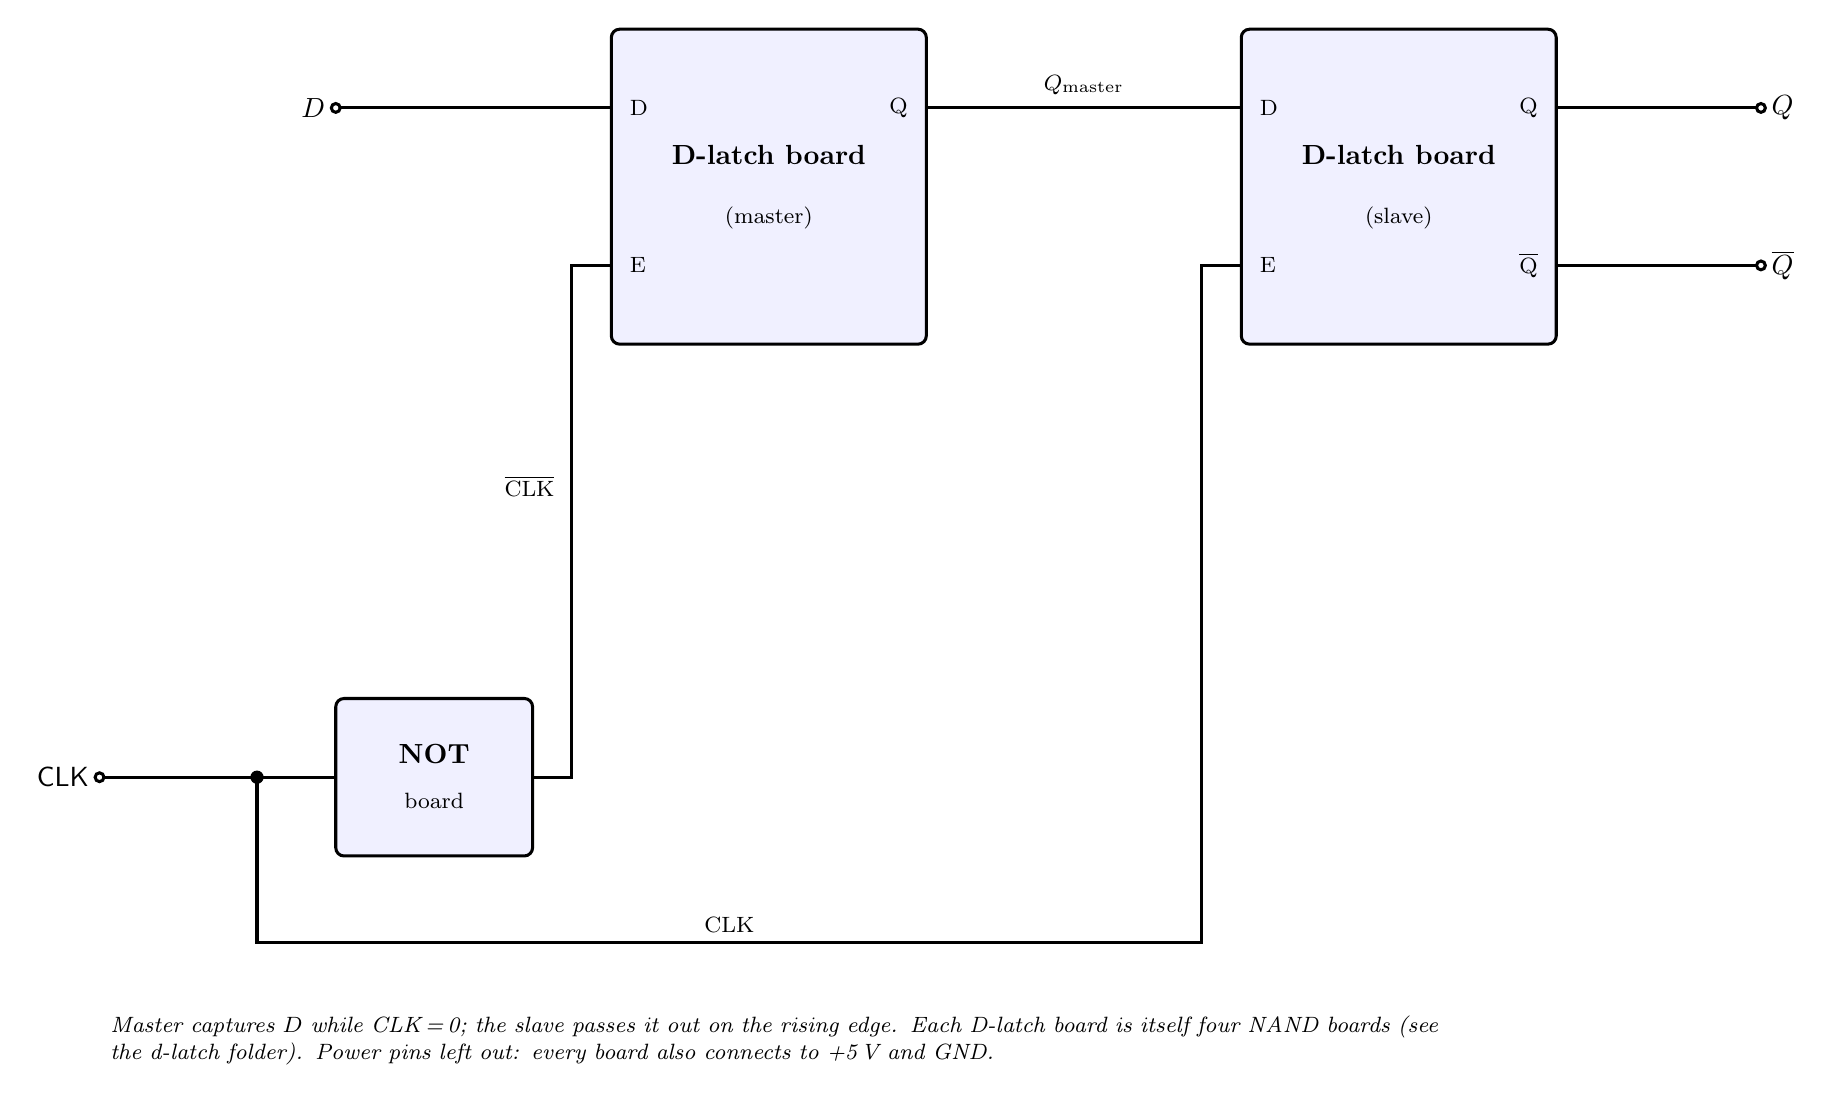
\begin{tikzpicture}[line width=1.1pt, font=\sffamily]

  % ---------- two D-latch boards ----------
  \draw[brd] (5.0,3.0) rectangle (9.0,7.0);
  \node[font=\bfseries] at (7.0,5.4) {D-latch board};
  \node[font=\footnotesize] at (7.0,4.6) {(master)};
  \draw[brd] (13.0,3.0) rectangle (17.0,7.0);
  \node[font=\bfseries] at (15.0,5.4) {D-latch board};
  \node[font=\footnotesize] at (15.0,4.6) {(slave)};

  \node[anchor=west,font=\footnotesize] at (5.1,6.0){D};  \node[anchor=west,font=\footnotesize] at (5.1,4.0){E};
  \node[anchor=west,font=\footnotesize] at (13.1,6.0){D}; \node[anchor=west,font=\footnotesize] at (13.1,4.0){E};
  \node[anchor=east,font=\footnotesize] at (8.9,6.0){Q};
  \node[anchor=east,font=\footnotesize] at (16.9,6.0){Q}; \node[anchor=east,font=\footnotesize] at (16.9,4.0){$\overline{\mathrm Q}$};

  % ---------- D input, master Q -> slave D, outputs ----------
  \draw (1.5,6.0) node[ocirc]{} node[left]{$D$} -- (5.0,6.0);
  \draw (9.0,6.0) -- (13.0,6.0);  \node[anchor=south,font=\footnotesize, fill=white, inner sep=1.5pt] at (11.0,6.1){$Q_{\mathrm{master}}$};
  \draw (17.0,6.0) -- (19.6,6.0) node[ocirc]{} node[right]{$Q$};
  \draw (17.0,4.0) -- (19.6,4.0) node[ocirc]{} node[right]{$\overline{Q}$};

  % ---------- clock + NOT board ----------
  \draw[brd] (1.5,-3.5) rectangle (4.0,-1.5);
  \node[font=\bfseries] at (2.75,-2.2){NOT}; \node[font=\footnotesize] at (2.75,-2.8){board};
  \draw (-1.5,-2.5) node[ocirc]{} node[left]{CLK} -- (0.5,-2.5) coordinate (clk);
  \fill (clk) circle (2.4pt);
  \draw (clk) -- (1.5,-2.5);                                   % CLK -> NOT input

  % CLK-bar -> master E : step right clear of the board, then straight up
  \draw (4.0,-2.5) -- (4.5,-2.5) -- (4.5,4.0) -- (5.0,4.0);
  \node[anchor=east,font=\footnotesize, fill=white, inner sep=1.5pt] at (4.35,1.2) {$\overline{\mathrm{CLK}}$};

  % CLK -> slave E : down, along the bottom, up (its own clear lane)
  \draw (clk) -- (0.5,-4.6) -- (12.5,-4.6) -- (12.5,4.0) -- (13.0,4.0);
  \node[anchor=south,font=\footnotesize, fill=white, inner sep=1.5pt] at (6.5,-4.55) {CLK};

  \node[anchor=north west,font=\footnotesize\itshape,text width=17cm] at (-1.5,-5.4)
        {Master captures $D$ while CLK\,=\,0; the slave passes it out on the rising edge.
         Each D-latch board is itself four NAND boards (see the d-latch folder). Power pins
         left out: every board also connects to +5\,V and GND.};

\end{tikzpicture}
\end{document}
